\documentclass[a4paper,11pt]{article}

\usepackage[T1]{polski}
\usepackage[utf8]{inputenc}
\usepackage{graphicx}


\hoffset=-3.0cm                 
\textwidth=18cm                
\evensidemargin=0pt
\voffset=-3cm                  
\textheight=27cm                
\setlength{\parindent}{0pt}             
\setlength{\parskip}{\medskipamount}    
\raggedbottom                           

\title{Projekt indywidualny}
\author{Smoliński Mateusz}
\date{20.12.2022}

\begin{document}
\maketitle
\thispagestyle{empty}

\section{Cel dokumentu}
Celem dokumentu jest przedstawienie sprawozdania z wykonanego projektu w ramach przedmiotu Projekt Indywidualny. Opiekunem projektu jest Pan dr inż. Radosław Roszczyk.

\section{Cel projektu}
Celem projektu było wykonanie aplikacji - mapy myśli pozwalającej na przedstawienie pomysłów w postaci graficznych ikonek (dalej nazywanymi elementami) z tekstowmi notatkami ułożonych na płaszczyźnie (nazywaną planszą). Aplikacja ma umożliwiać użytkownikowi manipulację tych elementów, intuicyjne i responsywne poruszanie się po nich oraz możliwość zapisywania ich stanu na zewnętrznym serwerze.

\section{Użyte narzędzia}
W ramach projektu zostały użyte następujące narzędzia:
\begin{itemize}
    \item python3, kivy, gql - do wykonania apikacji klienta, przygotowania GUI i komunikacji z endpointem graphQL
    \item python3, flask, graphene, mongoengine - do postawienia niezależnego serwera, udostępnienia endpointa dla klienta, przetworzenia danych, przygotowania i komunikacji z bazą danych
    \item MongoDB - nie-SQLowa dokumentowa baza danych posiadająca podstawową funkcjonalność grafową użyta do przechowywania zestawów plansz
    \item VS Code - edytor tekstu
    \item git - narzędzie do kontroli wersji
\end{itemize}

\section{Rezultat projektu}

\subsection{Baza danych}
Do przechowywania zapiów użytkownika aplikacji została użyta baza danych MongoDB. Każdy z elementów jest zagnieżdżony (EmbeddedDocument) w planszy, a plansze są zagnieżdżone w zestawach plansz. Zastosowanie EmbeddedDocument spowodowane jest tym, że elementy/plansze są czytane/zapisywane tylko podczas używania całej planszy/zestawu plansz.

\subsection{Serwer}
W ramach projeku została przygotowana w pythonie aplikacja serwera przy użyciu frameworka flask. Udostęnia ona klientowi jeden graphQLowy endpoint przyjmujący CRUDowe zapytania do zestawów plansz i wykonuje je na bazie danych. Do poprawnego przygotowania zapytań i mutacji zostało wykorzystane narzedzie GraphiQL pozwalające je testować na lokalnej maszynie. Modele do bazy danych przygotowane są przy użyciu modułu mongoengine, który też steruje czytaniem, zapisywaniem i usuwaniem dokumentów z kolekcji.

\subsection{Aplikacja klient}
Aplikacja klienta została napisana w pythonie z użyciem modułu kivy za pomocą którego został wykonany interfejs użytkownika. Po uruchomieniu aplikacji pojawia się okno w którego centrum znajduję się domyślna, pusta plansza.

\begin{center}
    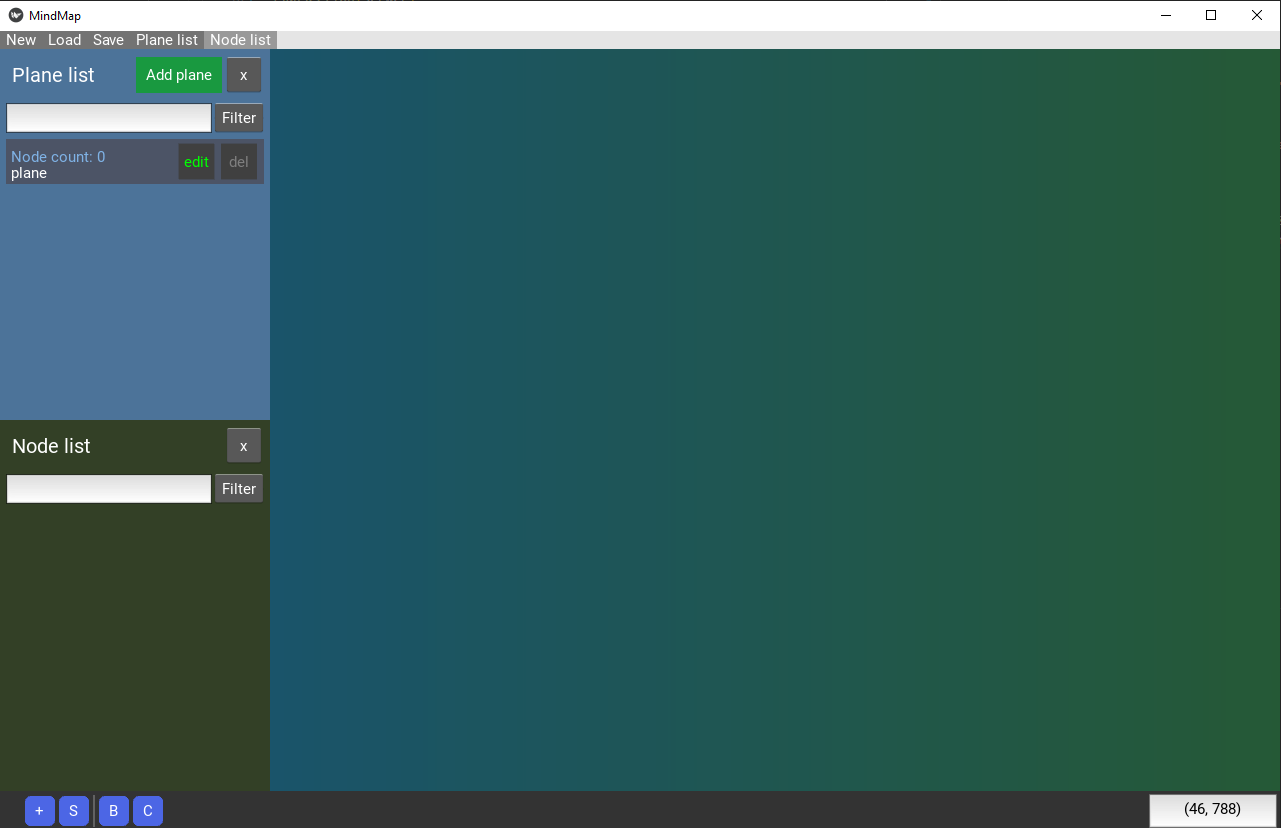
\includegraphics[width=16cm]{img/main_screen.png}
\end{center}

Widoczne na ekranie panele/opcje to:

\begin{itemize}
    \item na górze - opcje stworzenia nowej paczki, wczytania, zapisu, przełączanie list plansz i elementów
    \item po lewej - jeżeli są otwarte wyświetlają się listy plansz i elementów. Możliwość filtrowania po nazwie, zamknięcia listy (otworzyć ją ponownie możemy z górnego panelu). Z tego okna możemy przełączać pomiędzy planszami w paczce lub wybierać elementy.
    \item na dole - przycisk plus - jeżeli jest wybrany to kolejne kliknięcie na planszy stworzy nowy element i go automatycznie wybierze; przycisk - B (border) przełącza podświetlanie obszaru zakresu planszy; po prawej stronie - aktualna pozycja kursora względem planszy.
\end{itemize}

Po planszy poruszamy się za pomocą myszy, możemy ją przeciągać, przybliżać i oddalać.

\subsection{Edycja plansz i elementów}
Po wciśnięciu przycisku "Add plane" pojawi się okno dialogowe z możliwością edycji nazwy i rozmiaru pplanszy. Jeżeli kryteria (alfanumeryczna ze znakami podłogi i minusa, unikalna dla paczki nazwa, rozmiary w zakresie 1 <= x <= 10000 pikseli) są spełnione wciśnięcie przycisku Create storzy nową planszę, do której możemy się przełączyć na panelu listy plansz. W podobny sposób możemy te parametry zmieniać dla istniejących plansz wybierając opcję "edit". Jeżeli nie jest to aktywnie wybrana plansza, to możemy je też usunąć.

\begin{center}
    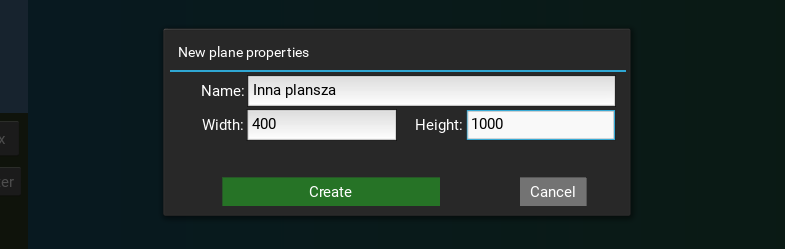
\includegraphics[width=12cm]{img/createpopup.png}
\end{center}

Elementy możemy umieszczać na planszy, zmieniać ich nazwę i opis oraz je usuwać. Klknięcie na element na planszy lub na liście wybiera go, co podświetla go w obu miejscach i wyświetla prawy panel umożliwiający jego edycję. Jednocześnie tylko jeden element może być w ten sposób wybrany. Najechanie na element na planszy lekko go podświetla i wyświetla okienko z jego nazwą i opisem.

\begin{center}
    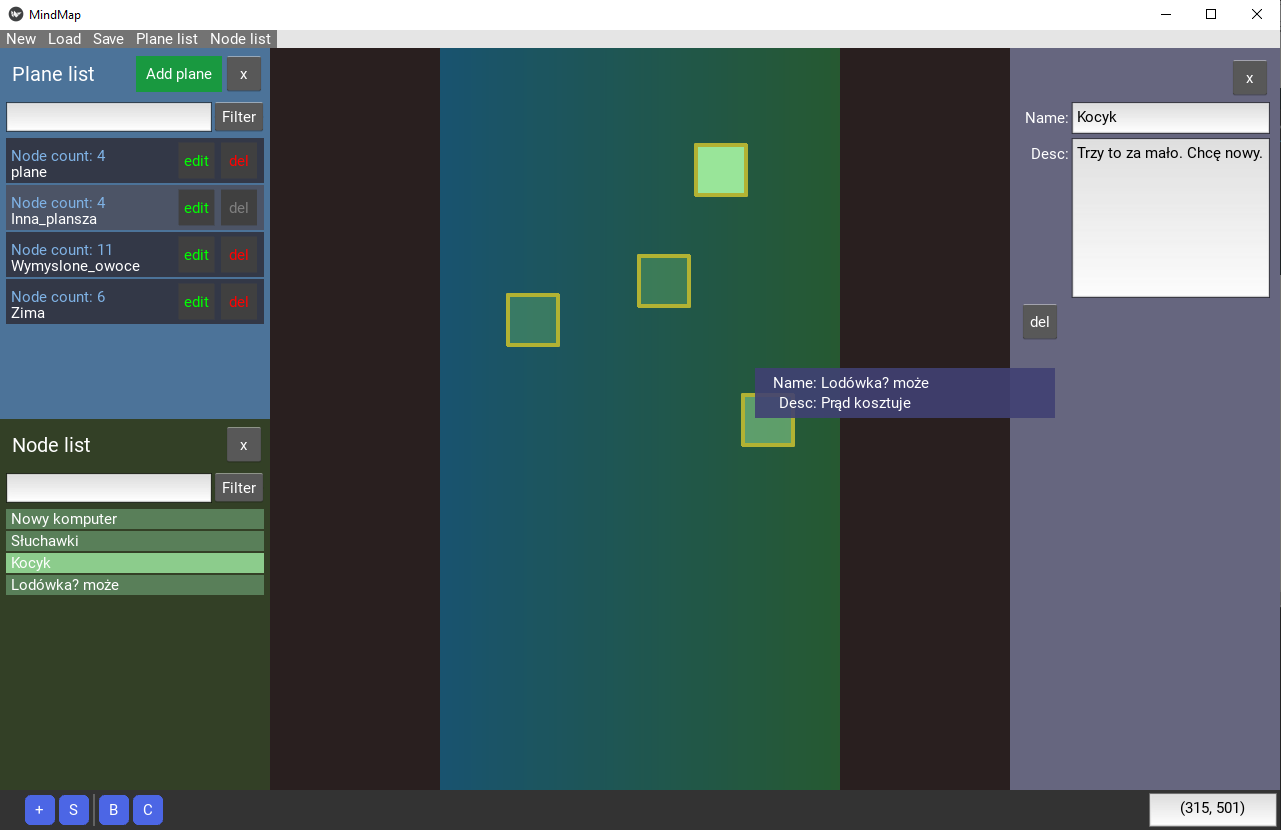
\includegraphics[width=16cm]{img/screen_with_things.png}
\end{center}

\subsection{Zapisywanie i wczytywanie}

Po wybraniu dowolnej opcji, która zamknęła by dotyczasową paczkę plansz, to znaczy "New", "Load" albo zamknięcia aplikacji pojawi się komunikat o to czy chcemy zapisać obecny stan. Wybranie opcji save wyświetli okno z możliwością wyboru zapisu na serwerze lub lokalnie (niezaimplementowane). Po wybraniu opcji zapisu na serwerze aplikacja podejmie próbę odczytania widniejących już tam zapisów. W przypadku niepowodzenia pojawi się stosowny komunikat.

\begin{center}
    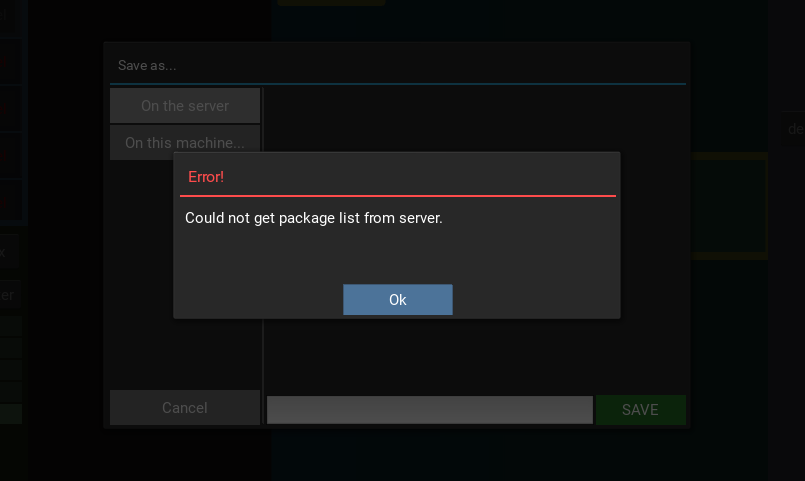
\includegraphics[width=13cm]{img/unsuccessfulsave.png}
\end{center}

Powtórne wybranie opcji serwera ponowi próbę wyświetlenia listy. Z tego miejsca możemy zobaczyć nazwy zapisanych w bazie danych paczek plansz, które możemy usnuąć. Podajemy nową nazwę i zapisujemy paczkę. Jeżeli spróujemy zapisać ją pod użytą już nazwą aplikacja zapyta użytkownika czy chcę nadpisać zapis. Po udanym zapise możemy przejść do analogicznie wyglądającej opcji LOAD i podejrzeć widniejący tam nowy zapis.

\begin{center}
    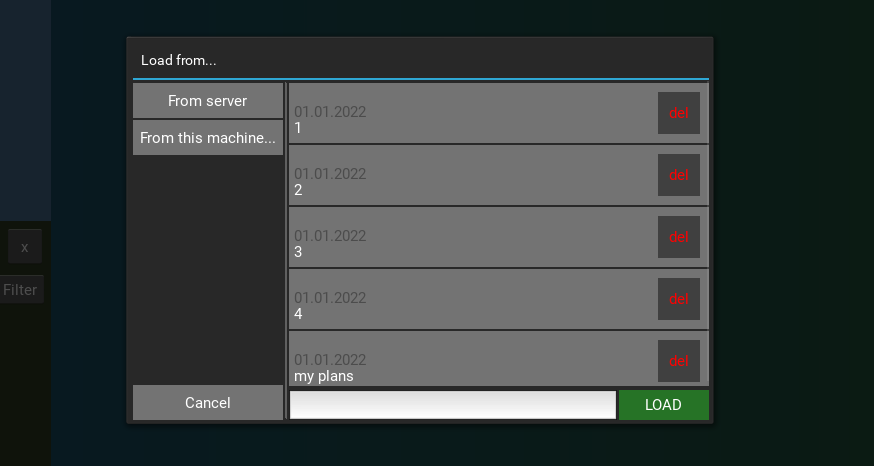
\includegraphics[width=13cm]{img/load.png}
\end{center}

Planszę możemy wczytać i kontynuować z zapisanego wcześniej stanu.

\section{Dalsze możliwości rozwoju}
Kolejnym krokiem byłoby dodanie możliwości przesuwania i edytowania wyglądu elementów, łączenie ich krawędziami i dodakowe opcje przełączania między planszami. Podczas wykonywania projektu nauczyłem się o innm języku do API niż REST - graphQL, tworzenia aplikacji z graficznym interfejsem, używania specjalnych widżetów (poruszająca się plansza, okienko poruszjące się wraz z kursorem, przeliczanie współrzędnych dla innych widżetów między oknem a planszą).

\end{document}